\externaldocument{../3/chapter_modeling}
\externaldocument{../5/chapter_implementation}
\externaldocument{../appendix/chapter_app}
\startchapter{Communication Identification}
\label{chapter:alo}
The goal of this work is to identify the communications from the dual\_trace. A dual\_trace is a pair of assembly level execution traces of two interacting programs. In this chapter, I discuss the characteristics of the execution trace and give the abstract definition of the dual\_trace and the execution trace. For all traces comply with this abstract trace definition, the analysis approach presented in this chapter can be applied for the communication identification.

The process of the communication identification is shown in Figure \ref{overview}. It takes the two traces $trace_0$ and $trace_1$ in the dual\_trace as input and output the identified communications. In this overview figure, there are four components. The function call event reconstruction component will take $trace_0$ and $trace_1$ as input and reconstruct the function call of interest from them respectively. The output sequences of events $etr_0$ and $etr_1$ will then flow into the stream extraction component separately. The stream extraction component will extract two sets of streams $str_0$ and $str_1$. Each stream in these two set corresponding to an endpoint of a communication. After that, the stream matching component will take both of the stream sets as input and try to match them by their channel identifiers and output the potential identified communications $cs$. Finally, the data verification component will verify each communication $c$ in this set and filter out those who doesn't satisfy the communication data preservation. The final output $cs'$ is the identified communications from the whole process. Algorithms are designed separately for each component.

\begin{figure}[H]
\centerline{\includegraphics[scale=0.6]{Figures/overview}}
\caption{Process of the Communication Identification from Dual\_trace}
\label{overview}
\end{figure}

\section{Dual\_Trace}
A dual\_trace consists of two assembly level execution traces of two interacting programs. There is no timing information of these two traces which means we don't know the timing relationship of the events of one trace with respect to the other. However the captured instructions in the trace are ordered in execution sequence. An execution trace consist of a sequence of instruction lines. Each instruction line contains the executed instruction, the changed memory, the changed registers, execution information. The execution information indicates the execution type which can be: Instruction, System call entry, System call exit, etc. For the execution type of system call entry and system call exit, system call Id is given in this information. With the system call id and the provided .dll files, a called system function name can be obtained. 

A dual\_trace is formalized as :

$dual\_trace = \lbrace trace_0, trace_1\rbrace$

where $trace_0$ and $trace_1$ are two assembly execution traces.

A trace is a sequence of executed instruction line. Hence, I define a $trace$ as a sequence of $n$ instruction lines:

$ trace = (l_1, l_2, ..., l_n)$ 

Each instruction line, $l$ is a tuple:

$l = <ins, mch, rch, exetype, syscallInfo>$

where $ins$ is the instruction, $mch$ is the memory changes, $rch$ is the register changes, $exetype$ is the execution type which can be instruction, system call entry, system call exit, and other types which are not concerned in this work, $syscallInfo = <exeName, offset>$ only appear when $exetype$ is system call entry or system call exit. $exeName$ is the executable file name(e.g. .dll and .exe), while $offset$ is the offset of the system function in this executable file.

Figure\ref{trace} is an example of a piece of execution trace complying to this definition. 

\begin{figure}[H]
\centerline{\includegraphics[scale=0.45]{Figures/trace}}
\caption{An example trace }
\label{trace}
\end{figure}

Figure\ref{executable} is an example of the information decoded from a executable file kernal32.dll. From this example we can see if an instruction line is a system call entry and its $syscallInfo = <kernal32.dll, 0x11870>$, this line is a function call to $copyFileExW$.

\begin{figure}[H]
\centerline{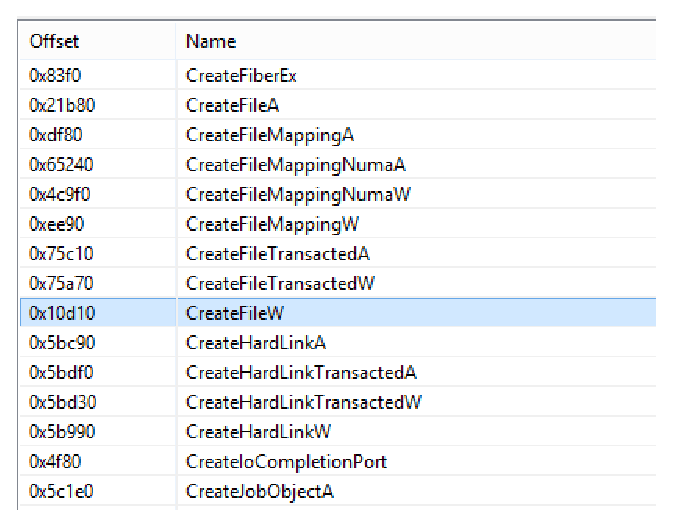
\includegraphics[scale=0.6]{Figures/executable}}
\caption{Information of kernal32.dll}
\label{executable}
\end{figure}

\section{Function Descriptor}
There would be lots of function calls in an execution trace. However, most of them are not of interest. We only concern the function call events of a specific communication method. To be able to identify and reconstruct the functions of interest, the function descriptions is required. Hence, I define the function descriptor as a set of function description:

$cdesc = \lbrace fdesc_1, fdesc_2,...,fdesc_p \rbrace$

Each element $fdesc$ can be defined as:

$fdesc = \lbrace name, type, inparamdesc, outparamdesc \rbrace$

where, $name$ is the function name, $type$ is the function type which can be one of the four types: $open$, $close$, $send$ and $receive$. $inparamdesc$ is the input parameter descriptions illustrating how the registers and memory contents map to a list of parameters of interest(you might not care for all parameters) of a given function call while $outparamdesc$ is the output parameter descriptions. 

Table\ref{functionexample} is an example of a function description. In this example, the function name is ReadFile, it is a function for data receiving, so that function type is $receive$. The parameter description includes the concerned parameters, which are Handle, RecvBuffer and MessageLength. The Handle is an input parameter which is a value stored in the register RCX. The RecvBuffer is an address for the input message stored in the register RAX. The MessageLength is a output value stored in register R9. The value of the input parameters can be retrieved from the memory state on the function call instruction line while the value of the output parameters can be retrieved from the memory state on the function return instruction line. If a parameter is an address instead of value, the address should be retrieved first, then the retrieved address should be used to find the buffer content in the memory state. The function description requires the understanding of the calling convention of the operating system. The Microsoft x64 calling convention can be found in Appendix \ref{convention}. More examples of communication method descriptions will be given in Chapter\ref{chapter:newsol}.

\begin{table}[H]
        \centering
        \caption{An example of a function description}
        \label{functionexample}
        \begin{tabular}{|l|l|l|l|l|l|l|l|}
            \hline
             \multirow{2}{*}{{\textbf{Name}}} & \multirow{2}{*}{{\textbf{Type}}} & \multicolumn{3}{c|}{\textbf{Input Parameter Description}} & \multicolumn{3}{c|}{\textbf{Output Parameter Description}} \\
              \cline{3-8} 
             & & \textbf{Name}& \textbf{Register} &  \textbf{Buffer/Value} & \textbf{Name}& \textbf{Register} &  \textbf{Buffer/Value}  \\
             \hline
             \multirow{2}{*}{ReadFile}
             &\multirow{2}{*}{receive} &  \multirow{2}{*}{Handle} & \multirow{2}{*}{RCX} & \multirow{2}{*}{Value} & RecvBuffer & RDX  & Buffer\\
              \cline{6-8} 
             & & & & & MessageLength & R9  & Value\\
            \hline            
        \end{tabular}
    \end{table}

\section{Function Call Event Reconstruction Algorithm}
In last two sections, I formalized the assembly execution trace and defined the function descriptor of a communication method. To be able to identify a communication, the elements consists a communication should be reconstruction from the traces first. To do so, we need to reconstruct the function call events, in which the function calls' parameters contain the information of a communication, such as the channel identifier, the packets send or received, etc. In this section, I define the function call event and present the algorithm to reconstruct the function call events from the assembly execution trace. 

With the function descriptor and the execution trace as input, the function call event reconstruction algorithm identifies function call entry instruction line and reconstruct the input parameters from the memory state of that line. Then it identifies the function call exit line of the corresponding function call and reconstruct the output parameters from the memory state of the function exit line. After iterate the whole execution trace, the algorithm outputs a sequence of function call events of size $m$ which can be defined as:

$etr = (ev_1, ev_2, ..., ev_m)$

A function call event $ev$ in $etr$ is defined as a triplet:

$ev = <funN, inparas, outparas, type>$

where $funN$ is the function name, $inparas$ includes all the input parameters with the parameter name and value while $outparas$ includes all the output parameters, and $type$ is the event type which inherit from the function description and can be one of the four types: $open$, $send$, $receive$ and $close$.

Note: If the parameter is an buffer, the parameter value is the string from the buffer instead of the buffer address.

An example of a sequence of function call events as the output of this algorithm is shown in Listing\ref{eventsexample}.

\begin{lstlisting}[caption= Example of  $etr$, label=eventsexample]
{funN:CreateNamedPipe, type:open,inparams:{Handler:18, FileName:mypipe}, outparams:{}},
{funN:CreateNamedPipe, type:open,  inparams:{Handler:27,  FileName:Apipe}, outparams:{}},
{funN:WriteFile, type:send, inparams:{Handler:27, SendBuf:Message1}, outparams:{MessageLen:9}},
{funN:WriteFile, type:send, inparams:{Handler:27, SendBuf:Message2}, outparams:{MessageLen:9}},
{funN:ReadFile, type:receive, inparams:{Handler:27}, outparams:{RecvBuf:Message3, MessageLen:9}},
{funN:CloseHandle, type:close, inparams:{Handler:27}, outparams:{}},
{funN:CloseHandle, type:close, inparams:{Handler:18}, outparams:{}}
\end{lstlisting}

Algorithm \ref{eventAlg} shows the detail of the function call event reconstruction algorithm. This algorithm is designed to reconstruct the function call events of a communication method. If multiple communication methods are under investigated, this algorithm can be run multiple times to achieve the goal. Since the function descriptions usually contain a  small number of concerned functions compared to the instruction line number in the execution trace, the time complexity of this algorithm is $O(N)$ , $N$ is the instruction line number of the trace.

\begin{algorithm}[H]
\DontPrintSemicolon
\caption{{\bf Function Event Reconstruction Algorithm} \label{eventAlg}}
\KwIn{ $trace, cdes$}
\KwOut{$etr$}
$etr \leftarrow \emptyset$\; 
Emulate the Execute of each instruction line of the trace;\;
\If{The instruction is a call to a function in the $cdes$}{
   Create an new function call event $ev$;\;
   $ev.funN  \leftarrow fdes.name$;\;
   $ev.type  \leftarrow fdes.type$;\;
   Append all the input parameters of interest to $ev.paras$;\;
   Continue the emulation until the function call return line;\;
   Append all the output parameters of interest to $ev.paras$;\;
   $etr.append(ev)$;\;
}
\KwRet $etr$;\;
\end{algorithm} 

\section{Channel Open Mechanisms}\label{mecha}
The channel open mechanism affect the event stream identification and event stream matching strategy. So I discuss them before presenting those algorithms. The channel open mechanism of named pipe and message queue is relatively simple. In windows implementation, only one function call is related to the handle identification of the stream. However, for TCP and UDP the mechanism is complicated.

\subsection{Named Pipe Channel Open Mechanisms} 
For Named Pipe communication method, a named pipe server is responsible for the creation of the pipe, while clients can connect to the pipe after it was created. The creation of a named pipe returns the handle of that pipe. So the identification of the stream only need to identify the pipe creation function call on the server side and the pipe connection function call on the client side. The handle returned by these function calls will be used later when data is being sent or received to a specified pipe. Figure\ref{namedpipeopen} exemplify the channel set up process for a Named Pipe communication in Windows. 

\begin{figure}[H]
\centerline{\includegraphics[scale=0.5]{Figures/namepipechannelopen}}
 \caption{Channel Open Process for a Named Pipe in Windows}
\label{namedpipeopen}
\end{figure}
    
\subsection{Message Queue Channel Open Mechanisms} 
For the Message Queue communication method, the endpoints of the communication can create the queue or use the existing one. However, both endpoints have to open the queue before they access it. The handle returned by the open queue function will be used later when messages are being sent or received to identify the queue. Figure\ref{msmqopen} exemplify the channel set up process for a Message Queue communication in Windows.
\begin{figure}[H]
\centerline{\includegraphics[scale=0.5]{Figures/msmqchannelopen}}
 \caption{Channel Open Process for a Message Queue in Windows}
\label{msmqopen}
\end{figure}

\subsection{UDP and TCP Channel Open Mechanisms} 
For UDP and TCP communication methods, the communication channel is set up by both endpoints of UDP and TCP channels. The function \textit{socket} should be called to create their own socket on both endpoints. After the socket handles are created, the server endpoint binds the socket to its service address and port by calling the function \textit{bind}. Then the server endpoint calls the function  \textit{accept} to accept the client connection. The client will call the function \textit{connect} to connect to the server. When the function \textit{accept} return successfully, a new socket handle will be generated and returned for further data transfer between the server endpoint and  the connected client endpoint. After all these operations are performed successfully, the channel is established and the data transfer can start. During the channel open stage, server endpoint has two socket handles, the first one is used to listen to the connection from the client, while the second one is created for real data transfer. Figure\ref{channelopen2} exemplify the channel open process for TCP and UDP  in Windows.
    
\begin{figure}[H]
\centerline{\includegraphics[scale=0.6]{Figures/tcpudpchannelopen}}
 \caption{Channel Open Model for TCP and UDP in Windows}
\label{channelopen2}    
\end{figure}

\section{Event Stream Extraction Algorithm}
The function call events in the $etr$ may belong to different endpoint. An event stream is a size $k$ sequence of function call events corresponding to an endpoint of a communication which can be defined as:

$s = (ev_1, ev_2, ..., ev_k)$

$s$ contains the channel open function call events, data send function call events, data receive function call events and channel close function call events. According to the channel open mechanisms discussed in Section\ref{mecha}, the identifier of the channel and the handle of the endpoint can be retrieved from the channel open function call events, while the data streams of the endpoint can be received from send function call events and data receive function call events. So that, given the stream $s$, the endpoint $ e =<handle,  d_r, d_s>$ and the $ch$ of a communication $c$ defined in a communication in Chapter\ref{chapter:mod} can be retrieved.

Note: the definition of $ev$ in $s$ is identical to that in $etr$. However, the event numbering of $s$ is different from $etr$. For example, $ev_1$ in $s$ and $ev_1$ in $etr$ might be different events.

The event stream extraction algorithm is designed to extract the streams from the sequence of function call events. In this algorithm, the stream is need to be identified by the channel open function calls first. Then all other events will be added to the stream.

The input of this algorithm is $etr$ from the function event reconstruction algorithm in Algorithm \ref{eventAlg}. Since the events in $etr$ are reconstructed in sequence of the instructions which are order by the time of occurrence, the events are implicitly sorted by time of occurrence. 

The output of this algorithm is a set of stream of size $p$, which can be defined as:

$str = (s_1, s_2, ..., s_p)$

As to the channel open mechanisms, two different algorithms are designed, one is for Name pipe and Message Queue, while the other is for TCP and UDP. 

\subsubsection{Event Stream Extraction Algorithm for Named Pipe and Message Queue}
This algorithm is designed for extraction of the streams for Named Pipe and Message Queue. Since for each endpoint of the communication, only one channel open function call is needed to identify the endpoint, it is simple to identify the stream once channel open function call event that create the endpoint handle is found. 

The same handle may be reused by other endpoint. However, reuse of the handle would not happen before this stream was closed by the channel close function call event. Therefore, before the detection of the channel close function call, if a new channel open function call with the same returned handle is detected, the second channel open will be ignored. This algorithm handle this by having the $tempstream$ set to keep track of the streams that are still open. Once the stream was closed, the handle can be used by another stream. The time complexity of this algorithm is $O(N)$ , $N$ is the number of events in the trace.

\begin{algorithm}[H]
\DontPrintSemicolon
\caption{{\bf Event Stream Exatraction Algorithm for Named Pipe and Message Queue} \label{streamext1}}
\KwIn{$etr$}
\KwOut{$str$} 
$str \leftarrow \emptyset$\; 
$tempstreams \leftarrow \emptyset$   
\For{$ev \in etr$}{
   $h \leftarrow$the handle identifier from $ev.paras$;\;
   \If{$ev.type = open$}{
      \If{$tempstreams[h]$ not exist}{
         $tempstreams[h] \leftarrow$ a new $s$;\;
         $tempstreams[h].append(ev)$;\;
      }     
   }
   \If{$ev.type = send$ Or $ev.type = receive$}{      
      \If{$tempstreams[h]$ exist}{
         $tempstreams[h].append(ev)$;\;
      }
   }
   \If{$ev.type = close$}{
      \If{$tempstreams[h]$ exist}{
         $tempstreams[h].append(ev)$;\;
         $str.append(tempstreams[h])$;\;        
         remove $tempstreams[h]$ from $tempstreams$;\;
      }
   }         
}
\KwRet $str$;\;
\end{algorithm} 

\subsubsection{Event Stream Extraction Algorithm for TCP and UDP}
This algorithm is designed for extraction of the event streams for TCP and UDP. In the channel open stage, a socket handle created by function call of $socket$ in both client and server. In the server side, this created socket is only used for listening to the client's connection. The listening is accomplished by calling the function $accept$. The input of the $accept$ function call is the listening socket handle, and the output of it is a new data transmission socket handle. This two socket handles are considered to be two handles for two streams, the stream identified by the listening handle is called the parent stream and the one identified by the data transmission handle is called the child stream. However the events in the parents stream contain the information needed for event stream matching algorithm later, so the children stream will inherit all the events from their parents. The time complexity of this algorithm is also $O(N)$, $N$ is the number of events in the trace.

\begin{algorithm}[H]
\DontPrintSemicolon
\caption{{\bf Event Stream Exatraction Algorithm for TCP and UDP} \label{streamext2}}
\KwIn{$etr$}
\KwOut{$str$} 
$str \leftarrow \emptyset$\; 
$tempstreams \leftarrow \emptyset$\;
\For{$ev \in etr$}{
   \If{$ev.funN = socket$}{
      $h \leftarrow$ the handle identifier from $ev.paras$;\;
      \If{$tempstreams[h]$ not exist}{
         $tempstreams[h] \leftarrow$ a new $s$;\tcp*[f]{new a stream}\;
         $tempstreams[h].append(ev)$;\;
      }     
   }  
   \If{$ev.funN = bind$ or $ev.funN = connect$}{
      $h \leftarrow$ the handle identifier from $ev.paras$;\;
      \If{$tempstreams[h]$ exist}{
         $tempstreams[h].append(ev)$;\;
      }     
   }   
   \If{$ev.funN = accept$}{
      $h \leftarrow$ the input listening handle in $ev.paras$;\tcp*[f]{handle of parent stream}\; 
      $hc \leftarrow$ the output data transfer handle in $ev.paras$;\tcp*[f]{handle of child stream}\; 
      \If{$tempstreams[h]$ exist}{  
        \If{$tempstreams[hc]$ not exist}{
            $tempstreams[hc] \leftarrow$ a new $s$;\tcp*[f]{a new stream for the child}\; 
        }
         $tempstreams[hc].append(tempstreams[h])$;\tcp*[f]{append parent's events}\;           
         $tempstreams[hc].append(ev)$;\tcp*[f]{append the current event}\;  
      }     
   }     
   \If{$ev.type = send$ Or $ev.type = receive$}{  
      $h \leftarrow$ the handle identifier from $ev.paras$;\;    
      \If{$tempstreams[h]$ exist}{
         $tempstreams[h].append(ev)$;\;
      }
   }
   \If{$ev.type = close$}{
      $h \leftarrow$ the handle identifier from $ev.paras$;\;
      \If{$tempstreams[h]$ exist}{
         $tempstreams[h].append(ev)$;\;
         $str.append(tempstreams[h])$;\;        
         remove $tempstreams[h]$ from $tempstreams$;\;
      }
   }         
}
\KwRet $str$;\;
\end{algorithm} 


\section{Event Stream Matching Algorithm}\label{streammatch}
The function event extraction algorithm and the event stream extraction algorithms all work on a single execution trace. To identify the communications from the dual\_trace, I need to match two event streams out of those extracted streams from each trace of the dual\_trace. The stream matching algorithm in this section is designed for this purpose. The inputs of the stream matching algorithm are two set of streams $str_0$ and $str_1$ which are output by the event stream extraction algorithm. The output of this algorithm is the matching set. Each matched item in this set contains two streams. 

This matching algorithm is not fully reliable. There are two situations which false negative error might emerge. Take Named Pipe for example, the first situation is multiple(more than two) interacting programs shared the same file as their own channel. Even though the channels are distinct for each communication, but the file is the same one. For example, the Named Pipe server is connected by two clients using the same file. In the server trace, there are two streams found. In each client trace, there is one stream found. For the dual\_trace of server and client1, there will be two possible identified communications, one is the real communication for server and client1 while the other is the false negative error actually is for server and client2. The stream in client1's trace will be matched by two streams in the server's trace. The second situation is the same channel is reused by the different endpoints in the same programs. For example, the Named Pipe server and client finished the first communication and then closed the channel. After a while they re-open the same file again for another communication. The matching is based on the identifiers. So that in this case, there will be two matching. Similar situations can also happen in Message Queue, TCP and UDP communication methods. The data stream verification algorithm discussed in Section\ref{verfication} can reduce the false negative errors. 

The stream matching depends on channel open mechanisms which are different from communication method to communication method. For TCP and UDP the matching can be considered as local address and port of server endpoint matching with remote address and port of client endpoint. For Named Pipe, it uses the file name, while for Message Queue, it uses the queue name as the identifier for matching of two streams. 

The following two subsections discuss the two matching algorithms, one is for Named Pipe and Message Queue, while the other is for TCP and UDP. For both of the algorithms, the time complexity of this algorithm is $O(N*M)$, $N$ and $M$ are the number of streams in both traces.

\subsection{Event Stream Matching Algorithm for Named Pipe and Message Queue}
For Named Pipe and Message Queue, the first function call event $ev_1$ in $s$ is the channel open function which is meaningful for endpoint handle identification. The channel identifier parameter can be found in the $ev_1.paras$. The identifier for Named Pipe is the file name of the pipe while for Message Queue is the queue name. This algorithm finds out all the possible communications regardless some of them might be false negative errors. The input $str_0$ and $str_1$ are two set of streams from the two traces of the dual\_trace. The output $ms$ is a set of two matching streams.

\begin{algorithm}[H]
\DontPrintSemicolon
\caption{{\bf Event Stream Matching Algorithm for Named Pipe and Message Queue} \label{matchAlg1}}
\KwIn{$str_0, str_1$}
\KwOut{$ms$}
$ms \leftarrow \emptyset$\; 
\For{$s_0 \in str_0$}{
\tcc{The first event is the open event}
   $id_0 \leftarrow$ get the channel identifier from $str_0[0].paras$;\;
   \For{$s_1 \in str_1$}{
      $id_1 \leftarrow$ get the channel identifier from $str_1[0].paras$;\;
     \If{$id_0 = id_1$}{
            $c.s_0 = s_0$;\;
            $c.s_1 = s_1$;\;
            $ms.append(c)$;\; 
      }
   }
}
\KwRet $ms$;\;
\end{algorithm} 

\subsection{Event Stream Matching Algorithm for TCP and UDP}
For TCP and UDP, multiple function calls collaborate to create the final communication channel. The local address and port of the server endpoint and the remote address and port of the client endpoint are used to identify the channel. This algorithm gets the local address and port of from the events in the stream of the server and remote address and port from the events in the stream of the client. Then it tries to match two streams by comparing the local and remote address and port. 

\begin{algorithm}[H]
\DontPrintSemicolon
\caption{{\bf Event Stream Matching Algorithm for TCP and UDP} \label{matchAlg2}}
\KwIn{$str_0, str_1$}
\KwOut{$cs$}
$cs \leftarrow \emptyset$\; 
\For{$s_0 \in str_0$}{ 
   $socketev_0 \leftarrow$ the $socket$ function call event from $str_0$;\;   
   $bindev_0 \leftarrow$  the $bind$ function call event from $str_0$;\;
   $connectev_0 \leftarrow$  the $connect$ function call event from $str_0$;\;
   \For{$s_1 \in str_1$}{
      $socketev_1 \leftarrow$ the $socket$ function call event from $str_1$;\;
      $bindev_1 \leftarrow$  the $bind$ function call event from $str_1$;\;
      $connectev_1 \leftarrow$  the $connect$ function call event from $str_1$;\;
\tcp*[f]{$socket$ function call event exists for both server and client streams, $bind$ function call event only exist for server streams while $connect$ function call event only exist for client streams}\;   
     \If{$socketev_0 !=null$ AND $socketev_1 != null$}{ 
\tcp*[f]{$s_0$ is a sever stream, $s_1$ is a client stream}\;
       \If{$bindev_0 != null$ AND $connectev_1 != null$}{
           $localServerAddr \leftarrow$ get serverAddr from $bindev_0.paras$;\;
           $remoteServerAddr \leftarrow$ get serverAddr from $connectev_1.paras$;\; 
       }
\tcp*[f]{$s_1$ is a sever stream, $s_0$ is a client stream}\;
       \ElseIf{$bindev_1 != null$ AND $connectev_0 != null$}{
           $localServerAddr \leftarrow$ get serverAddr from $bindev_1.paras$;\;
           $remoteServerAddr \leftarrow$ get serverAddr from $connectev_0.paras$;\; 
       }
       \If{$localServerAddr = remoteServerAddr$}{                  
            $c.s_0 = s_0$;\;
            $c.s_1 = s_1$;\;
            $cs.append(c)$;\;
          }
       }
    }
 }
\KwRet $cs$;\;
\end{algorithm}

\section{Data Stream Verification Algorithm}\label{verfication}
The data stream verification aims to verify if the data streams of the matched event streams align with the communication properties of the communication model in Chapter\ref{chapter:mod}. The data transfer characteristics divided the communications into reliable and unreliable categories. Named Pipe and TCP fall in the reliable category while Message Queue and UDP fall in the unreliable one. The properties of the models consists of content preservation and timing preservation. So that the verification should cover both preservations: 
\begin{itemize}
\item verify the content preservation of the data in the matched streams. 
\item verify the timing preservation of the data in the matched streams. 
\end{itemize}

To verify the timing preservation, the relative time of the events in both streams is needed. Unfortunately, we can only determine the relative time with in a stream but not crossing two streams. So that it's impossible to verify the timing preservations no matter for reliable or unreliable communications. The verification algorithms discussed in this section will only cover the content preservation.  

The inputs of the data stream verification algorithms are two preliminary matched streams $s_0$ and $s_1$. The output is the a boolean indicating if the streams satisfy the content preservation. All communications don't satisfy the content preservation should be excluded.

For each communication method the verification of the corresponding preservation is applied, That is, for Named Pipe and TCP, the reliable communication preservation need to be verified and for Message Queue and UDP, the unreliable communication preservation need to be verified. The following sub sections present the versification  algorithms for these four communication methods. In each sub section, I discuss the data transfer properties and scenarios of the communication method and then present the developed verification algorithm.

\subsection{Data Stream Verification Algorithm for Named Pipe}
A named pipe provides FIFO communication mechanism for inter-process communication. It can be a one-way or a duplex pipe. \cite{khambattinamed}

The basic data transfer characteristics of Named Pipe are:
\begin{itemize}
  \item Bytes are received in order
  \item Bytes sent as a segment can be received in multiple segments(the opposite is not true)
  \item No data duplication
  \item If a sent segment is loss, all the following segments will lost(this happen when the receiver disconnect from the channel) 
  
\end{itemize}

Based on these characteristics, the data transfer scenarios of Named pipe can be exemplified in Figure\ref{namedpipe}. 
\begin{figure}[H]
\centerline{\includegraphics[scale=0.4]{Figures/namedpipe}}
\caption{Data Transfer Scenarios for Named Pipe}
\label{namedpipe}
\end{figure}

The content preservation verification is trivial as comparing the concatenation of the packet content of the sent events in a stream to the the concatenation of the packet content of the receive events in the other stream, which is presented in Algorithm \ref{channelopen2}. Since the concatenation need to go through the events in the streams, the time complexity of this algorithm is also $O(N)$, $N$ is the total number of data transfer events in the two streams.

\begin{algorithm}[H]
\DontPrintSemicolon
\caption{{\bf Data Stream Verification of Named Pipe} \label{dataAlg1}}
\KwIn{$s_0, s_1$}
\KwRet{$satisfied$}\;
$send_0 \leftarrow$ concatenation of the payload of send function call events in $s_0$;\;
$send_1 \leftarrow$ concatenation of the payload of send function call events in $s_1$;\;
$receive_0 \leftarrow$ concatenation of the payload of receive function call events in $s_0$;\;
$receive_1 \leftarrow$ concatenation of the payload of receive function call events in $s_1$;\;
\If{$receive_1$ is prefix of $send_0$ AND $receive_0$ is prefix of $send_1$ }{
   \KwRet True;\;
}
\Else{
    \KwRet False;\;
}
\end{algorithm} 

\subsection{Data Stream Verification Algorithm for TCP}
TCP is the most fundamental reliable transport method in computer networking. TCP provides reliable, ordered, and error-checked delivery of a stream of octets between applications running on hosts in an IP network. The TCP header contains the sequence number of the sending octets and the acknowledge sequence this endpoint is expecting from the other endpoint(if ACK is set). The re-transmission mechanism is based on the ACK. 

The basic data transfer characteristics of TCP are:
\begin{itemize}
  \item Bytes received in order
  \item No data lost(lost data will be re-transmitted)
  \item No data duplication
  \item Bytes sent in packet and received in packet, no re-segmentation
\end{itemize}

Based on these characteristics,  the data transfer scenarios of TCP can be exemplified in Figure\ref{tcp}.
\begin{figure}[H]
\centerline{\includegraphics[scale=0.4]{Figures/tcp}}
 \caption{Data Transfer Scenarios for TCP}
\label{tcp}
\end{figure}

Regrading to the data transfer properties of TCP, the verification can be restricted to packet to packet. If all the send and receive events of the two streams can be matched, we can assert that the content preservation are satisfied. The verification algorithm of TCP is presented in Algorithm \ref{dataAlg2}. The time complexity of this algorithm is also $O(N)$, $N$ is the number of data transfer events in a stream.

\begin{algorithm}[H]
\DontPrintSemicolon
\caption{{\bf Data Stream Verification of TCP} \label{dataAlg2}}
\KwIn{$s_0, s_1$}
\KwRet{$satisfied$}\;
$sends_0 \leftarrow$ all sent events of $s_0$ in sequence;\;
$sends_1 \leftarrow$ all sent events of $s_1$ in sequence;\;
$receives_0 \leftarrow$ all receive events of $s_0$ in sequence;\;
$receives_1 \leftarrow$ all receive events of $s_1$ in sequence;\;
\If{$sends_0.size != receives_1.size$ Or $sends_1.size != receives_0.size$ }{
   \KwRet False;\;
}
\For{$i \in {0..sends_0.size}$}{
     \If{$sends_0[i].payload != receives_1[i].payload$}{
       \KwRet False;\;
   }
}
\For{$i \in {0..sends_1.size}$}{
     \If{$sends_1[i].payload != receives_0[i].payload$}{
       \KwRet False;\;
   }
}
 \KwRet True;\;
\end{algorithm} 



\subsection{Data Stream Verification Algorithm for Message Queue}
Message Queuing is a communication method to allow applications which are running at different times across heterogeneous networks and systems that may be temporarily offline can still communicate with each other. Messages are sent to and read from queues by applications. Multiple sending applications can send messages to and multiple receiving applications can read messages from one queue.\cite{redkar2004pro} In this work, only one sending application versus one receiving application case is considered. Multiple senders to multiple receivers scenario can be divided into multiple sender and receiver situation. Both applications of a communication can send to and receive from the channel.

The basic data transfer characteristics of Message Queue are:
\begin{itemize}
  \item Bytes sent in packet and received in packet, no bytes re-segmented
  \item Packets can lost
  \item Packets received in order
  \item No data duplication
\end{itemize}
Based on these characteristics, the data transfer scenarios of Message Queue can be exemplified in Figure\ref{msmq}.
\begin{figure}[H]
\centerline{\includegraphics[scale=0.4]{Figures/msmq}}
\caption{Data Transfer Scenarios for Message Queue}
\label{msmq}
\end{figure}

To verify the content preservation of the unreliable communication, Algorithm \ref{dataAlg3} tries to find the match sent packet in the other stream for each received packet. If any of the received packet can not be match, the content preservation is not satisfied. Since the sent packets are received in order, the searching for each received packet will start from the next index of the last matching sent packet. 

\begin{algorithm}[H]
\DontPrintSemicolon
\caption{{\bf Data Stream Verification of Message Queue } \label{dataAlg3}}
\KwIn{$s_0, s_1$}
\KwRet{$satisfied$}\;
$sends_0 \leftarrow$ all sent events of $s_0$ in sequence;\;
$sends_1 \leftarrow$ all sent events of $s_1$ in sequence;\;
$receives_0 \leftarrow$ all receive events of $s_0$ in sequence;\;
$receives_1 \leftarrow$ all receive events of $s_1$ in sequence;\;
\If{$sends_0.size < receives_1.size$ Or $sends_1.size < receives_0.size$ }{
   \KwRet False;\;
}
$lastMatchIndex = 0$;\;
\For{$i \in {0..receives_1.size}$}{
     $tempIndex = lastMatchIndex$;\;
     \For{$j \in {lastMatchIndex+1..sends_0.size}$}{
             \If{$sends_0[j].payload = receives_1[i].payload$}{
                      $lastMatchIndex = j$;\;
                      break the inner For loop;\;
            }  
     }   
\tcp*[f]{This received packet can not be matched by any sent packet}\;      
     \If{$tempIndex = lastMatchIndex$}{
                      \KwRet False;\;
            }     
}     
$lastMatchIndex = 0$;\;
\For{$i \in {0..receives_0.size}$}{
     $tempIndex = lastMatchIndex$;\;
     \For{$j \in {lastMatchIndex+1..sends_1.size}$}{
             \If{$sends_1[j].payload = receives_0[i].payload$}{
                      $lastMatchIndex = j$;\;
                      break the inner For loop;\;
            }  
     }   
     \If{$tempIndex = lastMatchIndex$}{
                      \KwRet False;\;
            }     
}  
 \KwRet True;\;
\end{algorithm} 

The time complexity of this algorithm is $O(N^2+M^2)$, $N$ and $M$ are the numbers of data sent events of the two streams.

\subsection{Data Stream Verification Algorithm for UDP}
UDP is a widely used unreliable transmission method in computer networking. It is a simple protocol mechanism, which has no guarantee of delivery, ordering, or duplicate protection. This transmission method is suitable for many real time systems. 

The basic data transfer characteristics of UDP are:
\begin{itemize}
  \item Bytes sent in packet and received in packet, no re-segmentation
  \item Packets can lost
  \item Packets can be duplicated
  \item Packets can arrive receiver out of order
\end{itemize}

Based on these characteristics, the data transfer scenarios of UDP can be exemplified in Figure\ref{upd}.
\begin{figure}[H]
\centerline{\includegraphics[scale=0.4]{Figures/udp}}
 \caption{Data Transfer Scenarios for UDP}
\label{upd}
\end{figure}

Similar to Message Queue, Algorithm \ref{dataAlg4} try to find the match sent packet in the other stream for each received packet. If any of the received packet can not be match, the content preservation is not satisfied. However, due to the disordering can happen in UDP, the searching for each received packet will not constraint the searching index. But the matched sent packet will excluded from the following searching, which means each sent packet can only match to one received packet.

\begin{algorithm}[H]
\DontPrintSemicolon
\caption{{\bf Transmitted Verification of UDP} \label{dataAlg4}}
\KwIn{$s_0, s_1$}
\KwRet{$satisfied$}\;
$sends_0 \leftarrow$ all sent events of $s_0$ in sequence;\;
$sends_1 \leftarrow$ all sent events of $s_1$ in sequence;\;
$receives_0 \leftarrow$ all receive events of $s_0$ in sequence;\;
$receives_1 \leftarrow$ all receive events of $s_1$ in sequence;\;
\If{$sends_0.size < receives_1.size$ Or $sends_1.size < receives_0.size$ }{
   \KwRet False;\;
}
\For{$i \in {0..receives_1.size}$}{
    $matchFlag = False$;\;
     \For{$j \in {0..sends_0.size}$}{
             \If{$sends_0[j].payload = receives_1[i].payload$}{
                      $matchFlag = True$;\;
                      delete the packet from $sends_0$
                      break the inner For loop;\;
            }  
     }   
\tcp*[f]{This received packet can not be matched by any sent packet}\;      
     \If{$matchFlag = False$}{
                      \KwRet False;\;
            }     
}     
\For{$i \in {0..receives_0.size}$}{
    $matchFlag = False$;\;
     \For{$j \in {0..sends_1.size}$}{
             \If{$sends_1[j].payload = receives_0[i].payload$}{
                      $matchFlag = True$;\;
                      delete the packet from $sends_0$
                      break the inner For loop;\;
            }  
     }   
     \If{$matchFlag = False$}{
                      \KwRet False;\;
            }     
} 
 \KwRet True;\;
\end{algorithm} 

The time complexity of this algorithm is $O(N^2+M^2)$, $N$ and $M$ are the numbers of data sent transfer events in the two streams.

\section{Communication Identification Process}
The general communication identification of the dual\_trace consist of the algorithms presented previously in this chapter and can be summarized as the follow steps with the corresponding algorithm for each communication categories(i.e. reliable or unreliable) and each communication methods:

\textbf{Step 1.} Execute the Function Event Reconstruction algorithm to the two traces in the dual\_trace

\textbf{Step 2.} Execute the Stream Exaction Algorithm to the both traces 

\textbf{Step 3.} Use the Stream Matching Algorithm to match the streams of the two traces

\textbf{Step 4.} Verify the matched streams by the their satisfaction of the content preservation

\textbf{Step 5.}  Include the matched streams that satisfy the preservation

\textbf{Step 6.}  Retrieve the endpoint $e =<handle,  d_r, d_s>$ and channel identifier $ch$ from the matched streams and output a set the communications. (No corresponding algorithm for this step since the retrieval is only reorganize the information in the streams and is trivial)


\section{Limitation of the Identification}
The Identification discussed in this chapter is not perfect. It has two major limitations:
\begin{itemize}
    \item The timing preservation of the communication is not verified.
    \item Due to the data transmitted in two communications can be identical(or their difference can not be tell by the content verification), the false negative error of the identification can not be eliminated. Figure\ref{secondlevelmatching} indicates the ineffective and effective identification scenarios. 
\end{itemize}



\begin{figure}[H]
\centerline{\includegraphics[scale=0.5]{Figures/secondlevelmatching}}
 \caption{Communication Identification Scenarios}
\label{secondlevelmatching}
\end{figure}



